\documentclass[12pt]{article}
\usepackage[english,german]{babel}
\usepackage[utf8]{inputenc}
\usepackage{color}
\usepackage{hyperref}
\usepackage{mathtools}
\usepackage{graphicx}

\setlength{\parindent}{0em} 
\hypersetup{
    colorlinks=true,
    linktoc=all,
    linkcolor=black,
    urlcolor=black
}
%Gummi|065|=)
\title{\Huge\textbf{Bioinformatik von RNA- und Proteinstrukturen}}
\author{}
\date{}

% set title of table of contents
\renewcommand*\contentsname{Inhalt}

% https://www.sharelatex.com/learn
% http://www.math.ubc.ca/~cautis/tools/latexmath.html
% http://www.golatex.de/wiki/Kategorie:Befehlsreferenz
% https://en.wikibooks.org/wiki/LaTeX/Mathematics

\begin{document}

\begin{titlepage}

\maketitle
\thispagestyle{empty}
\end{titlepage}
\newpage

\begin{titlepage}
\tableofcontents
\thispagestyle{empty}
\end{titlepage}
\newpage

\section{Formale Sprachen}

Formale Sprache\footnote{\url{https://de.wikipedia.org/wiki/Formale\_Sprache}}
L über Alphabet $\Sigma$\\
L $\subseteq$ $\Sigma$*\\
% @todo: URL kleensche Hülle korrigieren
mit $\Sigma$* = Kleensche Hülle\footnote{\url{https://de.wikipedia.org/wiki/Kleenesche\_und\_positive\_H\%C3\%BClle}} von $\Sigma$\\


$$\Sigma^* = \bigcup_{n=0}^{\infty} \Sigma^{n}$$\\
$\Sigma^0 = \{\varepsilon\}, \Sigma^1 = \Sigma, \Sigma^2 = \Sigma \times \Sigma$\\
$\varepsilon \to$ leeres Wort (leere Menge)\\

Beispiel: $\Sigma = \{a\}, \Sigma^*=\{\varepsilon, a, aa, aaa, ...\}, L = \{a, aa, aaaa, ...\}$

\subsection{formale Grammatik G}

G = (N, $\Sigma$, P, S) mit\\
\begin{itemize}
	\item N = Nichtterminale
	\item $\Sigma$ = Alphabet
	\item P = Produktionsregeln
	\item S = Startsymbol ($\epsilon$ N)
\end{itemize}

% @todo: was bedeutet diese Zeile?
P $\subseteq (N \cup \Sigma)^* / N(N \cup \Sigma)^* \to (N \cup \Sigma)^*$\\
\\
Beispiel:\\
% @todo: die Produktionsregeln von links nach rechts anwenden wenn es mehrere gibt?
G=(\{S\}, \{a\}, $\{S \to aaS, S \to a\}$, S)\\
führt zu: S $\to$ aaS $\to$ aaa

\subsection{Klassifikation von formalen Sprachen}
durch die Comsky-Hierarchie\footnote{\url{https://de.wikipedia.org/wiki/Chomsky-Hierarchie}}:
\begin{itemize}
	\item Typ 0 = rekursiv auszählbar ($\alpha N \beta \to \gamma$)
	\item Typ 1 = kontext-sensitiv ($\alpha N \beta \to \alpha \gamma \beta$)
	\item Typ 2 = kontext-frei, N $\to (N \cup \Sigma)^* \to$ stochstisch kontextfreie Grammatik (SCFG) $\to$ Dynamics Programming
	\item Typ 3 = regular ($N \to \Sigma | \Sigma N$) $\to$ dann immer Hidden Markov Model (HMM) modellierbar
\end{itemize}

bei Alignments:
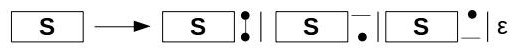
\includegraphics[width=0.7\textwidth]{rna_and_protein_src/1.jpg}
\\\\
Erweiterung mit Wahrscheinlichkeit:
G=(N, $\Sigma$, P, S, $\Omega$)\\
mit $\Omega$ = Wahrscheinlichkeit für Produktionsregeln\\
\\

\underline{jetzt auf RNA-Vorhersagen:}\\
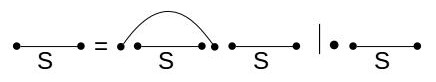
\includegraphics[width=0.7\textwidth]{rna_and_protein_src/2.jpg}

scoring scheme: Bewertung von 
$\sigma$ (
\includegraphics[width=0.05\textwidth]{rna_and_protein_src/4.jpg}) = 1, 
($\sigma$ (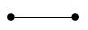
\includegraphics[width=0.05\textwidth]{rna_and_protein_src/3.jpg})), 
$\sigma$ (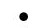
\includegraphics[width=0.05\textwidth]{rna_and_protein_src/5.jpg}) = 0\\
scoring function: max Basepairs: + (Summe), Anzahl der Strukturen: $\cdot$ (Multiplikation)
choice function: max Basepairs: max, Anazhl der Strukturen: + (Summe)

% @todo: Bild für Aufteilung der Fälle bei der RNA-Vorhersage
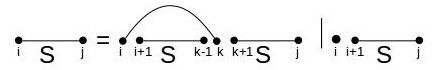
\includegraphics[width=0.7\textwidth]{rna_and_protein_src/6.jpg}

\subsection{Hidden Markov Model}

% Bild einfügen

M: Match, I: Insertion, D: Deletion\\

Grammatik:
\begin{itemize}
	\item M $\to M_{A\_A} | ... | I | D$
	\item I $\to I_{A\_\_} | ... | D | M$
	\item D $\to D_{\_\_A} | ... | M | I$
\end{itemize}

Beispiel:\\
% @todo: Beispiel einfügen

\underline{Faltungsgrammatik}\\\\
S $\to (S)S | .S| \varepsilon$\\
Nichtterminale = S, Alphabet = \{(, ), .\}\\
Beispiel in Baumdarstellung:
% @todo: Zeichnung einfügen

weiteres Beispiel: Sankoff, Kombination von zwei Grammatiken (Alignment und Faltung)\\\\
\underline{Alignmentgrammatik}\\\\
S $\to .S | \_S | \varepsilon$\\
G = $(N = \{S\}, \Sigma = \{., \_\}, P=\{S \to .S | \_S | \varepsilon\}, S)$\\
Alignment: $G^2 = G \times G = (N \times N, \Sigma \times \Sigma, P^2, (S,S))$\\
$P^2 = P \times P = 
\left(
    \begin{array}{c}
      S \\
      S
    \end{array}
  \right)
$

\section{Einleitung}

Struktur: Form $\rightarrow$ Funktion\\
Funktion folgt Form, Form folgt Sequenz\\
Proteine, RNA, DNA: Sequenzen\\
\\
\underline{4 Strukturlevels:}
\begin{itemize}
	\item primäre Struktur (Sequenz): 1 Dimension
	\item sekundäre Struktur (grobe Annäherung an Struktur): 2 Dimensionen
	\item tertiäre Struktur (räumliche Struktur): 3 Dimensionen
	\item quartiäre Struktur (räumliche Anordnung von interagierenden Strukturen): 4 Dimensionen
\end{itemize}

Behandlung hauptsächlich 2D

\section{Strukturvorhersage}

\subsection{Nussinov}

\subsection{Turner-Modell (Nearest-Neighbor-Modell)}

\subsection{Zuker-Algorithmus}

\subsubsection{suboptimales Falten}

\subsection{Wuchty-Algorithmus}

\subsubsection{Wuchty-Backtracking}

\subsection{McCaskill}

\subsection{stochastisches Backtracking}

\subsection{Strukturvorhersagen verbessern}

\subsection{Konsensusstrukturvorhersagen}

\subsection{Wie kann RNA evolvieren?}

\subsubsection{Neutrale Netzwerke}

\subsubsection{SHAPE-Abstraktion}

\subsubsection{Energielandschaften}

\subsubsection{Faltungskinetik}

\subsubsection{Barriers Trees}

\subsubsection{Flooding-Algorithmus}

\subsubsection{Co-transcriptional folding}

\end{document}